\documentclass[11pt,a4paper]{jsarticle}

\usepackage[dvipdfmx]{graphicx}
\usepackage{graphicx}
\usepackage[top=10truemm,bottom=20truemm,left=25truemm,right=25truemm]{geometry}
\usepackage{comment}

%
\title{前期実験報告書}
\author{東京大学工学部物理工学科 賀川研究室 平松信義}
\date{\today}
\begin{document}
\maketitle

\tableofcontents
\newpage

\section{はじめに}
\subsection{研究の背景}
\subsection{研究の目的}
\subsection{本論文の構成}
この報告書の筆者は2018年前期の卒業研究において、偏光顕微光学系の設計と作成を行った。またIrTe$_2$のバルク試料の相転移を、抵抗測定と偏光顕微鏡像から観察した。

\section{実験方法}
IrTe$_2$試料は理化学研究所の星谷研究員から提供を受けた。
\begin{figure}[htbp]
  \begin{center}
   \includegraphics[width=100mm]{sample.eps}
  \end{center}
  \caption{ディフューザーあり}
  \label{fig:sample}
\end{figure}

\subsection{抵抗率の測定}
IrTe$_2$試料の抵抗を四端子法を用いて測定した。試料に四端子を接続する時の注意点を\ref{sec:4terminal}に示した。
抵抗値は

\subsection{光学顕微鏡}
顕微鏡を用いて、IrTe$_2$試料の反射率を顕微鏡で観察した。光学系をの模式図を図\ref{fig:microscope}に示す。
光学素子は光源とコリメータを除き、全てXYZステージの上に固定した。
\begin{figure}[htbp]
  \begin{center}
   \includegraphics[width=100mm,angle=270]{microscope.eps}
  \end{center}
  \caption{ディフューザーあり}
  \label{fig:microscope}
\end{figure}


\section{実験結果}
\subsection{抵抗測定}
\begin{figure}[htbp]
  \begin{center}
   \includegraphics[width=100mm]{resistance.eps}
  \end{center}
  \caption{ディフューザーあり}
  \label{fig:resistance}
\end{figure}

\subsection{光学顕微鏡}
\subsubsection{300K}
\begin{figure}[htbp]
 \begin{minipage}{0.333\hsize}
  \begin{center}
   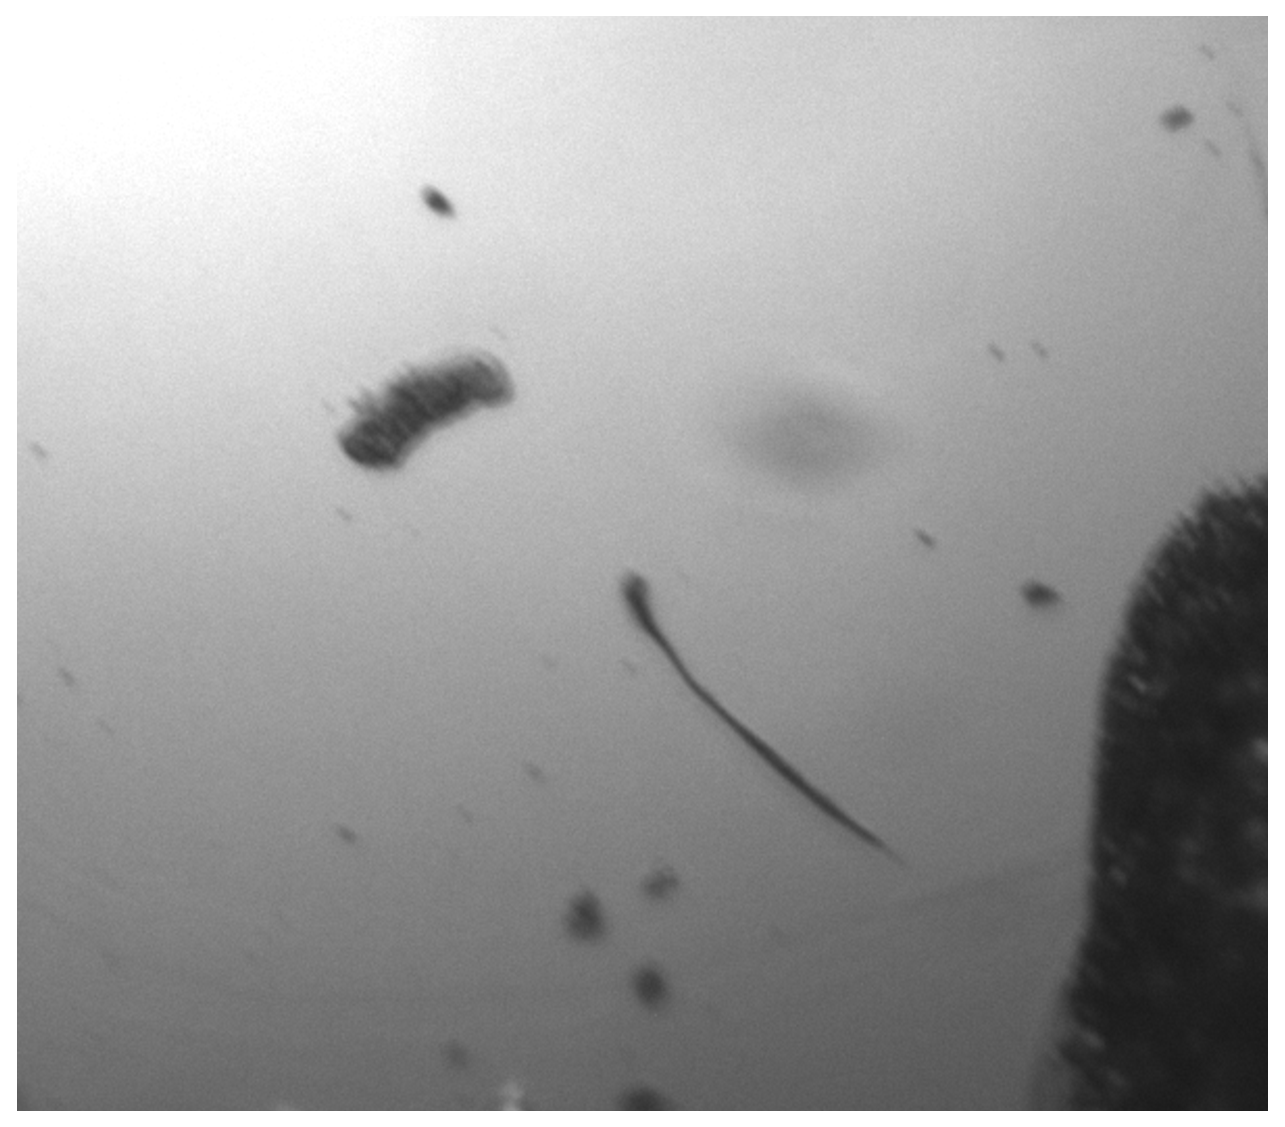
\includegraphics[width=\hsize]{nonpol300.eps}
  \end{center}
  \caption{無偏光}
  \label{fig:nonpol300}
 \end{minipage}
 \begin{minipage}{0.333\hsize}
  \begin{center}
   \includegraphics[width=\hsize]{hh300.eps}
  \end{center}
  \caption{平行偏光(x偏光/x検出)}
  \label{fig:hh300}
 \end{minipage}
 \begin{minipage}{0.333\hsize}
  \begin{center}
   \includegraphics[width=\hsize]{vv300.eps}
  \end{center}
  \caption{平行偏光(y偏光/y検出)}
  \label{fig:vv300}
 \end{minipage}
\end{figure}
\begin{figure}[htbp]
 \begin{minipage}{0.333\hsize}
  \begin{center}
   \includegraphics[width=\hsize]{vh300.eps}
  \end{center}
  \caption{直交偏光(y偏光/x検出)}
  \label{fig:vh300}
 \end{minipage}
 \begin{minipage}{0.333\hsize}
  \begin{center}
   \includegraphics[width=\hsize]{hv300.eps}
  \end{center}
  \caption{直交偏光(x偏光/y検出)}
  \label{fig:hv300}
 \end{minipage}
 \begin{minipage}{0.333\hsize}
  \begin{center}
   \includegraphics[width=\hsize]{vh300_subtractedby_hv300.eps}
  \end{center}
  \caption{図\ref{fig:vh300}と図\ref{fig:hv300}の差分}
  \label{fig:vh300_subtractedby_hv300}
 \end{minipage}
\end{figure}


\subsubsection{250K}
\begin{figure}[htbp]
 \begin{minipage}{0.333\hsize}
  \begin{center}
   \includegraphics[width=\hsize]{nonpol250.eps}
  \end{center}
  \caption{無偏光}
  \label{fig:nonpol250}
 \end{minipage}
 \begin{minipage}{0.333\hsize}
  \begin{center}
   \includegraphics[width=\hsize]{hh250.eps}
  \end{center}
  \caption{平行偏光(x偏光/x検出)}
  \label{fig:hh250}
 \end{minipage}
 \begin{minipage}{0.333\hsize}
  \begin{center}
   \includegraphics[width=\hsize]{vv250.eps}
  \end{center}
  \caption{平行偏光(y偏光/y検出)}
  \label{fig:vv250}
 \end{minipage}
\end{figure}
\begin{figure}[htbp]
 \begin{minipage}{0.333\hsize}
  \begin{center}
   \includegraphics[width=\hsize]{vh250.eps}
  \end{center}
  \caption{直交偏光(y偏光/x検出)}
  \label{fig:vh250}
 \end{minipage}
 \begin{minipage}{0.333\hsize}
  \begin{center}
   \includegraphics[width=\hsize]{hv250.eps}
  \end{center}
  \caption{直交偏光(x偏光/y検出)}
  \label{fig:hv250}
 \end{minipage}
 \begin{minipage}{0.333\hsize}
  \begin{center}
   \includegraphics[width=\hsize]{vh250_subtractedby_hv250.eps}
  \end{center}
  \caption{図\ref{fig:vh250}と図\ref{fig:hv250}の差分}
  \label{fig:vh250_subtractedby_hv250}
 \end{minipage}
\end{figure}

\subsubsection{50K}
\begin{figure}[htbp]
 \begin{minipage}{0.5\hsize}
  \begin{center}
   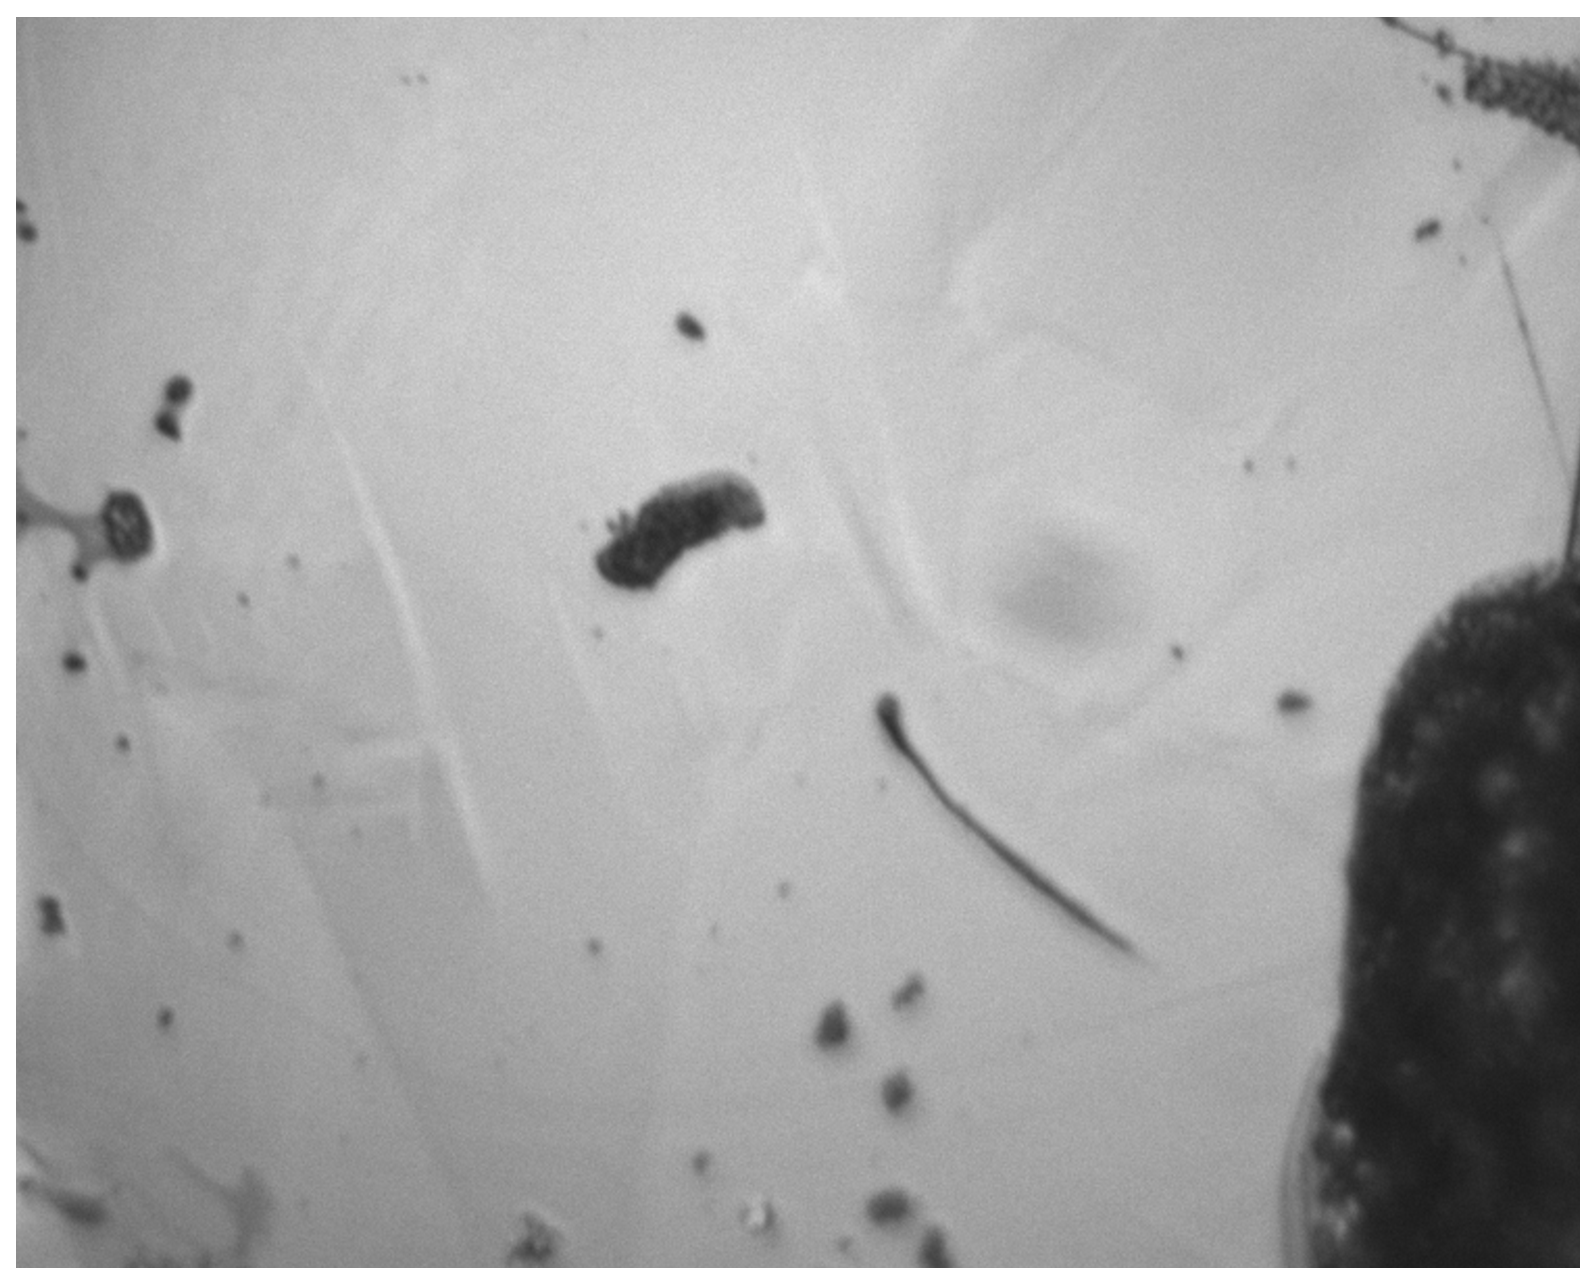
\includegraphics[width=\hsize]{nonpol50.eps}
  \end{center}
  \caption{無偏光}
  \label{fig:nonpol50}
 \end{minipage}
 \begin{minipage}{0.5\hsize}
  \begin{center}
   \includegraphics[width=\hsize]{vh50.eps}
  \end{center}
  \caption{直交偏光(y偏光/x検出)}
  \label{fig:vh50}
 \end{minipage}
\end{figure}

\section{議論}

\section{今後の課題と展望}


%\section{謝辞}
\newpage
\appendix
\section{顕微光学系に関する改良}
\subsection{光源とディフューザー}
\begin{figure}[htbp]
 \begin{minipage}{0.5\hsize}
  \begin{center}
   \includegraphics[width=70mm]{with_diffuser.eps}
  \end{center}
  \caption{ディフューザーあり}
  \label{fig:with_diffuser}
 \end{minipage}
 \begin{minipage}{0.5\hsize}
  \begin{center}
   \includegraphics[width=70mm]{without_diffuser.eps}
  \end{center}
  \caption{ディフューザーなし}
  \label{fig:without_diffuser}
 \end{minipage}
\end{figure}

\subsection{顕微光学系の偏光依存性}
非偏光ビームスプリッタと対物レンズに無偏光の光を銀ミラー上で反射し、検光子を回転したときの偏光依存性を図\ref{fig:objective}に示す。
\begin{figure}[htbp]
  \begin{center}
   \includegraphics[width=120mm]{objective.eps}
  \end{center}
  \caption{ディフューザーあり}
  \label{fig:objective}
\end{figure}

\subsection{非偏光ビームスプリッタの偏光依存する位相遅れ}
\begin{figure}[htbp]
  \begin{center}
   \includegraphics[width=120mm]{nonpol_BS.eps}
  \end{center}
  \caption{ビームスプリッタの偏光依存性}
  \label{fig:objective}
\end{figure}


\section{三斜晶の反射率}
\subsection{一般の場合の反射率テンソルの導出}
文献\cite{dielectric_tensor_triclinic}にしたがって、誘電率テンソルが与えられた場合の反射率を導く。

結晶中のMaxwell方程式は、
\begin{eqnarray}
\nabla \times {\bf E} = -\mu_0 \frac{\partial \bf B}{\partial t}\\
\nabla \times {\bf H} = -\epsilon_0 \epsilon  \frac{\partial \bf E}{ \partial t}.
\end{eqnarray}

二式をフーリエ変換すると、
\begin{eqnarray}
\label{E1}
{\bf k} \times {\bf E} = \mu_0 \omega {\bf H}\\
\label{H1}
{\bf k} \times {\bf H} = -\epsilon_0 \omega  \epsilon  {\bf E}.
\end{eqnarray}

式\ref{E1}に式\ref{H1}を代入してベクトル解析の公式を用いると、
\begin{eqnarray}
k^2 {\bf E} - ( {\bf k} \cdot {\bf E} ) {\bf k}=  k_0^2  \epsilon {\bf E}.
\end{eqnarray}
ただし$k_0=\omega \sqrt{\epsilon_0 \mu_0}$は自由空間の波数。

ここでxy平面への垂直入射を仮定して、$k_x=k_y=0, k_z=k$とする。このとき
\begin{eqnarray}
\left(
    \begin{array}{ccc}
      \epsilon_{xx}-p & \epsilon_{xy} & \epsilon_{xz} \\
      \epsilon_{yx} &  \epsilon_{yy} -p & \epsilon_{yz} \\
      \epsilon_{zx} & \epsilon_{zy} & \epsilon_{zz} \\
    \end{array}
\right)
\left( \begin{array}{c} E_x\\ E_y\\ E_z \\ \end{array} \right)
=\left( \begin{array}{c} 0\\ 0\\ 0 \\ \end{array} \right)
\end{eqnarray}
ここで$p=k^2/k_0^2$は自由空間の波数と結晶中の波数の比の二乗である。


三斜晶の空間群は$\rm P\overline{1}$であり、比誘電率テンソル$\epsilon$は対称テンソルである(ただし物質が磁性を持たず、外部磁場が印加されていないとした)。すなわち
\[
  \epsilon = \left(
    \begin{array}{ccc}
      \epsilon_{xx} & \epsilon_{xy} & \epsilon_{xz} \\
      \epsilon_{yx} & \epsilon_{yy} & \epsilon_{yz} \\
      \epsilon_{zx} & \epsilon_{zy} & \epsilon_{zz} \\
    \end{array}
  \right)
\]


\subsection{IrTe$_2$高温相の反射率テンソル}
三斜晶の空間群は$\rm P\overline{1}$
$\rm IrTe_2$は温度$280K$付近で構造相転移することが知られている。低温側で空間群$\rm P\overline{1}$の対称性をもち三斜晶となる。高温で空間群$\rm P\overline{3}m1$の対称性をもつ三方晶\cite{space_group_IrTe2}。

\subsection{IrTe$_2$低温相の反射率テンソル}
三斜晶の空間群は$\rm P\overline{1}$


\section{サンプルの端子付け}
\label{sec:4terminal}
本実験ではサンプルの温度依存する抵抗率を四端子法から測定するために、$IrTe_2$のサンプルとユニバーサル基板の間を金線を用いて電気的に接続した。
金線とサンプル、金線とユニバーサル基板の接続には銀ペーストを使った。
手順と端子付けの際に気をつけたことに関して、簡単にまとめる。

\subsection{端子づけに使った道具}

\begin{itemize}
\item 乾いた毛筆($250\mu m$程度)
\item 乾いた毛筆($500\mu m$程度)
\item 毛筆(銀ペースト用)
\item 毛筆(グリース用)
\item 銀ペーストを練るようじ
\item ピンセット
\item キムワイプ
\end{itemize}
*毛筆は用途によって印をつけておく(黒の塗りつぶし:銀ペースト;縞模様:細い)。毛は1mm程度の長さが良いと思う。長すぎると金線やサンプルを飛ばしてしまう。

そのほかの道具・材料
\begin{itemize}
\item 金線を切るためのハサミ
\item 金線を置いておくゴムマット
\item 銀ペーストを練るスライドガラス
\item サンプル近くに置く銀ペーストのパレット
\item サンプルとパレットを乗せるスライドガラス
\item ユニバーサル基板(ピッチ2.5mm)
\item 両面テープ
\item 金線(太さ250um)
\item 銀ペースト
\item 光学顕微鏡
\end{itemize}

毛筆の作り方
1. 二液式接着剤を混ぜてつまようじの先に薄くつける\\
2. 一本の毛(腕毛、すね毛、まつげ、髪の毛など)を、接着剤に先を出して埋め込む\\%
3. 接着剤が乾いたら、毛の長さをはさみで調整する\\


\subsection{作業を始める前に} 
\begin{itemize}
\item 前日はよく寝る
\item 机の上を整理整頓
\item 空調のスイッチを切る(作業終了後は再度スイッチを入れる)
\item 左右の接眼レンズの間隔とピントを調整する
\item 椅子の高さを調整
\end{itemize}

 
\subsection{作業の手順} 
サンプルに4つの端子をつける手順
1. 準備
\begin{itemize}
\item ユニバーサル基板を適当な大きさにカットする
\item スライドガラスに両面テープでユニバーサル基板を貼り付ける。このとき銀ペーストを伸ばすパレットを横に作る。
\item 金線を必要なぶん切っておく(まっすぐで長さのそろった、汚れていないものが扱いやすい)
\item 銀ペーストをよく練って、サンプル横のパレットに適量のせる
\end{itemize}
 
2. サンプルの取り付け
\begin{itemize}
\item 基板にグリースを毛筆で少量つける。毛筆で伸ばす必要はない
\item 毛筆の先にグリースを微量つけてサンプルを持ち上げ、ユニバーサル基板につけたグリースの上に置く
\item サンプルを上から軽く押して、密着させる
\end{itemize}
 
3. 電流端子2本の取り付け
\begin{itemize}
\item まず金線一本をピンセットと毛筆で移動する。一方の端がサンプルの近くで、もう一方がユニバーサル基板の銅箔の近くにくるようにする
\item 金線と銅箔を銀ペーストでくっつける。銀ペーストが固まる前に、サンプル側の端がサンプルに触れるように微調整する
\item もう一本の金線に関しても同様に、銅箔と金線を銀ペーストでくっつけて固まるまで待つ
\item 銅箔側の銀ペーストが固まったら、サンプルと金線を銀ペーストでつなぐ。流れる電流がなるべく一様な密度になるように、横に広く接続することを意識する
 \end{itemize}
 
4. サンプルの持ち上げ
\begin{itemize}
\item サンプルと金線の間の銀ペーストが固まったら、金線と基板の間に毛筆を入れてサンプルを持ち上げる
 \end{itemize}
 
5. 電圧端子2本の取り付け
\begin{itemize}
\item 電流端子と同様に接続する。ただし、銀ペーストがサンプルに触れる面積が小さくなるように心がける。また測定中の低温でユニバーサール基板や金線が収縮して、サンプルと接合点に強いテンションがかかるのを防ぐため、金線を銅箔につけて固めた後少し曲げるとよいと思う。
 \end{itemize}
 
6. そのほか端末の取り付け
\begin{itemize}
\item PPMSのための端末をつくる
\end{itemize}

7. %
\begin{itemize}
\item 記録のため写真をとっておく
\item 4端子間の抵抗を測定して2~3オーム程度であることを確認する
\end{itemize}
 

\subsection{作業が終わったら} 
\begin{itemize}
\item 空調の電源をオンにする
\item 顕微鏡の照明をオフにする
\item 机の上の片付け
\item サンプルをデシケータに入れる
\end{itemize}
 
 \subsection{作業のコツ} 
ピンセット
\begin{itemize}
\item 汚れたらキムワイプで拭いて先を綺麗に保つ
\item 金線はつよく掴まない、できるだけ平行につまむ
\item 先を保護するために、金線はゴムマットの上でつまむ
\end{itemize}
 
毛筆
\begin{itemize}
\item 銀ペーストを塗ったあとは毛を溶媒で洗って、キムワイプで拭く
\item つまようじを人差し指と中指で持つと疲れない
\item 小指の付け根を台につけて、左手を添えると震えにくい
キムワイプ
\item サンプルを汚してしまったら、キムワイプの先(繊維)でふき取るとよい
\end{itemize}
 
銀ペースト
\begin{itemize}
\item 溶媒(コハク酸ジエチル)の液溜まりと固い銀ペーストの塊はライドガラス上に離しておく。銀ペーストは少しずつ溶かして混ぜる。液溜まりでは銀ペーストを塗ったあとの毛筆を洗う。
\item パレットの銀ペーストは乾きやすいので、定期的に溶媒を足して練り直す
銀ペーストと金線
\item まず薄いペーストの表面張力で金線とサンプルをくっつける。乾くのを待って、濃いペーストで形を整える。はみ出した時は細く切った(2*20mm)キムワイプの先をちぎってねじったものに溶媒を含ませて拭く
顕微鏡の倍率
\item 高倍率で固定して、毛筆やピンセットはなるべく動かさない。スライドガラスとサンプルを動かすようにする
\end{itemize}
 
休憩
\begin{itemize}
\item 一時間半に少なくとも一度休憩するのが望ましい
\end{itemize}

四端子測定が上手くいかない時
\begin{itemize}
\item 光学顕微鏡像の画像をとって、測定前と比べてみる
\item 各端子間の抵抗を測ってみる
\item 毛筆で端子を触ってみる
\end{itemize}

\begin{comment}
\section{誘電率テンソル}
$\rm IrTe_2$は温度$280K$付近で構造相転移することが知られている。低温側で空間群$\rm P\overline{1}$の対称性をもち三斜晶となる。高温で空間群$\rm P\overline{3}m1$の対称性をもつ三方晶\cite{space_group_IrTe2}。

低温側でc軸(z方向にとる)に垂直な電場応答は以下の対称な誘電率テンソル$\epsilon_{LT}$で表される。\cite{dielectric_tensor_triclinic}
\[
  \epsilon_{LT} = \left(
    \begin{array}{cc}
      \epsilon_{xx} & \epsilon_{xy}\\
      \epsilon_{yx} & \epsilon_{yy}\\
    \end{array}
  \right)
\]

高温側でc軸に垂直な応答は以下の誘電率テンソル$\epsilon_{HT}$で表される。
\[
  \epsilon_{HT} = \left(
    \begin{array}{cc}
      \epsilon_{} & 0\\
      0 & \epsilon_{}\\
    \end{array}
  \right)
\]

これらの対称性を
\end{comment}

\section{光学クライオスタット}
\subsection{冷凍機}
Advenced Research Systems社の冷凍機(DE204)を用いた。

\subsection{真空引きポンプ}


\newpage
\bibliography{interim_report.bib}
\bibliographystyle{junsrt}


\end{document}
%コンパイルの仕方
%1. texファイルを一回コンパイル
%2. bibファイルを一回コンパイル
%3. texファイルを三回コンパイル